\section{Background}
\label{background}

%% \joerg{0.5 page: FDR, OSP; introduce nomystery running example for
%%   illustration, only goal facts (no action-set props), FDR then OSP
%%   simply not enough fuel}

%% \joerg{ijcai text snippets:}

We consider the \emph{finite-domain representation (FDR)} framework
\cite{backstrom:nebel:ci-95,helmert:ai-09}, with finite-domain state
variables.
%
An FDR task \defined{\task} is a tuple $\task =
(\vars,\acts,\cost,\init,\goal)$ where \vars\ is the set of
\defined{variables}, \acts\ is the set of \defined{actions}, $\cost:
\acts \mapsto \reals^+_0$ is the action \defined{cost} function,
\init\ is the \defined{initial state}, and \goal\ is the
\defined{goal}. A \defined{state}, in particular \init, is a complete
assignment to $\vars$; \goal\ is a partial assignment to \vars; each
action $a \in \acts$ has a \defined{precondition} $\pre_a$ and an
effect $\eff_a$, both partial assignments to \vars. We will refer to
variable-value pairs $v=d$ as \defined{facts}, and we will identify
partial variable assignments with sets of facts.
%
An action $a$ is \defined{applicable} in a state $s$ if $\pre_a
\subseteq s$. The outcome state $s\apply{a}$ is like $s$ except that
$s\apply{a}(v) = \eff_a(v)$ for those $v$ on which $\eff_a$ is
defined. The outcome state of an iteratively applicable action
sequence $\plan$ is denoted $s\apply{\plan}$.

We address an oversubscription variant of FDR, where an
\defined{oversubscription planning (OSP) task} is a tuple $\task =
(\vars,\allowbreak\acts,\allowbreak\cost,\allowbreak\init,\allowbreak\goalhard,\allowbreak\goalsoft,\allowbreak\costbound)$
like an FDR task but with two goals -- the \defined{hard} goal
\goalhard\ and the \defined{soft} goal \goalsoft, assumed to be
defined on disjoint sets of variables -- as well as an additional
\defined{cost bound} $\costbound \in \reals^+_0$. A \defined{plan} is
an action sequences \plan\ whose summed-up cost is $\leq \costbound$
and where $\goalhard \subseteq \init\apply{\plan}$. Good plans achieve
a ``maximally valuable'' subset of \goalsoft. OSP frameworks in the
literature employ measurements (\eg\ goal-fact rewards) of what it
means to be maximally valuable. Here we assume instead that the user's
preferences over the soft goals are difficult to specify and/or
elicitate, and planning is an iterative process as described by Smith
\shortcite{smith:aaai-12}. We are concerned with the analysis of
plan-property dependencies to support that process.

Note that this form of analysis makes sense for any planning task
whose goal facts cannot be achieved in conjunction, for reasons other
than a cost bound. In particular, planning with non-reproducible
resources is of interest if the resources are insufficient to achieve
all goals. With resources encoded as discrete FDR state variables,
this can be viewed as a special case of our OSP formulation. In our
experiments, we will consider the resource-constrained planning (RCP)
benchmarks by Nakhost et al.\ \shortcite{nakhost:etal:icaps-12}, which
allow to control resource constrainedness (basically the ratio between
available vs.\ required resource amounts).

%\begin{figure}[htb]
\begin{wrapfigure}{r}{0.45\columnwidth}
\vspace{-0.3cm} \hspace{-0.8cm} %
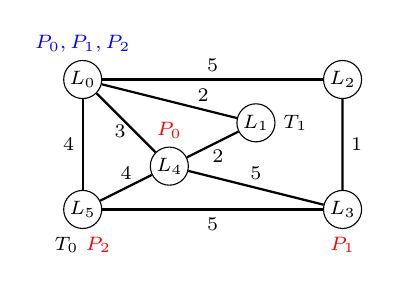
\begin{tikzpicture}[scale=0.55]
	\scriptsize
  \node[draw, circle, inner sep=1pt, label=above:{\textcolor{blue}{$P_0, P_1,P_2$}}] (l0) at (0,0) {$L_0$};
  \node[draw, circle, inner sep=1pt, label=right:{$T_1$}] (l1) at (4,-1) {$L_1$};
  \node[draw, circle, inner sep=1pt] (l2) at (6,0) {$L_2$};
  \node[draw, circle, inner sep=1pt, label=below:{\textcolor{red}{$P_1$}}] (l3) at (6,-3) {$L_3$};
  \node[draw, circle, inner sep=1pt, label=above:{\textcolor{red}{$P_0$}}] (l4) at (2,-2) {$L_4$};
  \node[draw, circle, inner sep=1pt, label=below:{$T_0$ \textcolor{red}{$P_2$}}] (l5) at (0,-3) {$L_5$};

  \draw[thick] (l0) to node[above] {5} (l2);
  \draw[thick] (l0) to node[above, pos=0.75] {2} (l1);
  \draw[thick] (l0) to node[below, pos=0.4] {3} (l4);
  \draw[thick] (l0) to node[left] {4} (l5);
  \draw[thick] (l2) to node[right] {1} (l3);
  \draw[thick] (l4) to node[below, pos=0.6] {2} (l1);
  \draw[thick] (l4) to node[above] {5} (l3);
  \draw[thick] (l5) to node[below] {5} (l3);
  \draw[thick] (l4) to node[above] {4} (l5);
\end{tikzpicture}
%\vspace{-0.25cm} \hspace{-0.6cm} \caption{Illustrative IPC NoMystery example.}
%\label{fig:nomystery-example}
\vspace{-0.3cm}
\end{wrapfigure}
%\end{figure}

For illustration, we will use an RCP running example from IPC
NoMystery, a transportation domain with fuel consumption. The
variables encode truck and package positions, actions drive trucks or
load/unload packages. Drive actions consume the fuel resource
associated with the respective truck. The amount of fuel consumed
depends on the road connection taken. As a concrete example task, we
will use the task with two trucks and three packages illustrated
above. Fuel costs are indicated at road segments. The packages are
initially at $L_0$ (shown in blue); their goal locations are $L_4$,
$L_3$,and $L_5$ (shown in red).
